%filters
\section{滤镜}
\subsection{模糊滤镜}
简单的模糊滤镜产生一种和相机快门失焦的相似效果,为了产生模糊的特效,该滤镜将该点的像素指和相邻的像素点的值求平均值作为该点的值.
\begin{description}
\item[优点]	计算速度快,适合大图像
\item[缺点]	它的效果在大图像中很难被感知,而在小图像中就很明显
\end{description}
\subsubsection{高斯模糊滤镜}\label{filters:blur:gaussian}
高斯滤镜是应用最广泛的一个模糊滤镜.该滤镜以最基础的方式使得图片更模糊.它能够在相对短的时间里产生一个非常模糊的效果.
高斯滤镜对每个活动图层或者选区都会产生效果,并且会对对话框里定义的范围里所有的像素求平均.\\
对话框参数设置:
\begin{description}
\item[模糊半径]	设置模糊的强烈程度--对于某个像素点,半径越大,求平均的点越多,图片就会越模糊.
\item[模糊方法]	GIMP支持两种高斯滤镜的方式:IIR和RLE.它们都能产生相同的结果,可是在不同情况下,两种方法处理的速度不一样
\begin{description}
\item[IIR]	无限脉冲响应滤波器(Infinite impulse response),该方法适合比较大的模糊半径以及不是电脑生产的图片
\item[RLE]	游程编码(Run-length encoding),该方法适合计算机生成的图片或者[those with large areas of constant intensity.]
\end{description}
\end{description}
高斯滤镜效果比对如下图\ref{filters:blur:gaussian:figure}:
\begin{figure}[!htbp]
	\centering
	\caption{高斯滤镜}
	\subfigure[原图]{
		\label{filters:blur:gaussian:figure:original}
    		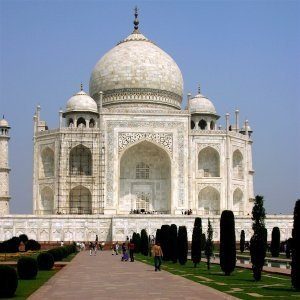
\includegraphics{figs/blur_gaussian_original.jpg}}
    	\subfigure[处理后]{
    		\label{filters:blur:gaussian:figure:dealt}
    		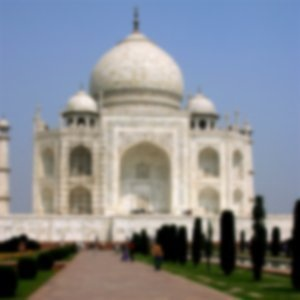
\includegraphics{figs/blur_gaussian_dealt.jpg}}
    	\label{filters:blur:gaussian:figure}
\end{figure}
\clearpage


\subsection{噪声滤镜}
噪声滤镜给可见图层或者选中的选区添加噪音\footnote{图像中各种妨碍人们对其信息接受的因素,详情见http://baike.baidu.com/view/944141.htm}。要是想要除去图片上的小噪点,可以使用降噪\ref{filters:enhance:despeckle}和选择高斯模糊滤镜\ref{filters:blur:selective_gaussian}。

\subsubsection{RGB噪声滤镜}\label{filters:noise:rgb}
RGB噪声滤镜可以给一个图层或一个选区添加符合正态分布的噪声。它利用RGB色彩模式来产生噪音(噪声直接加到每个像素的R,G,B的值上)。正态分布是指只有一小部分像素被很大的值影响,大部分像素只是增加了非常微小的噪声。(如果你对一个填充了灰色的图像进行RGB噪声滤镜后,再看它的直方图,你将看到一个典型的钟形高斯曲线)。而图像中是一个非常自然的噪声。\\
注:\textcolor{red}{该滤镜对索引图像没有效果。}\\
对话框参数设置:
\begin{description}
\item[噪声相关性]	噪声可能是不相关的(additive)或者是相关的(multiplicative - 也被称为斑点噪声)。选中该选项时,每个通道的值乘以一个正态分布值。所以噪声取决于通道值:更大的信道值会导致更多的噪音,而黑色(小值)倾向于保持黑色。
\item[RGB的一致性]	当此按钮被选中时,你可以单独移动每个RGB滑块。否则,三个滑块将一起移动。相关噪声将被添加到每个像素中的所有信道,所以像素的色调不会发生大的变化。
\end{description}
RGB噪声滤镜效果比对如下图\ref{filters:noise:rgb:figure}:
\begin{figure}[!htbp]
	\centering
	\caption{RGB噪声滤镜}
	\subfigure[原图]{
		\label{filters:noise:rgb:figure:original}
    		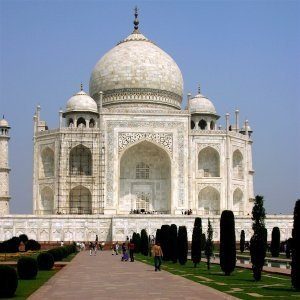
\includegraphics{figs/blur_gaussian_original.jpg}}
    	\subfigure[处理后]{
    		\label{filters:noise:rgb:figure:dealt}
    		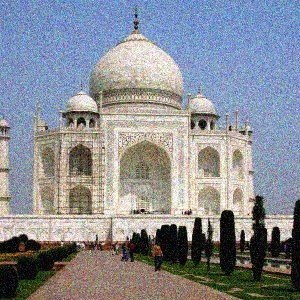
\includegraphics{figs/blur_rgb_dealt.jpg}}
    	\label{filters:noise:rgb:figure}
\end{figure}
\clearpage


\subsection{绘制滤镜}
GIMP的大部分滤镜是通过变换它们的内容作用在一个图层上,但是在绘制这个滤镜中有点不一样。它们从空白开始创建,大部分情况是删除在图层上的任何东西。一些滤镜创建随机或噪图案,其他一些滤镜创建重复的分形图案,还有一个Gfig滤镜是一个专门用来创建矢量图像的工具。

\subsubsection{拼图滤镜}\label{filters:render:pattern:jigsaw}
该滤镜将把你的图片转变成一个拼图。图片边缘有点失真,所以用平滑处理一下会让图片看得更好。\\
\underline{技巧}:如果你想要轻易的选择单个的拼图,你可以在一个填充了白色的单独图层上绘制拼图图案,并且设置图层模式为正片(multiply)。接着你就可以用魔术棒工具在新拼图图层上选择单个拼图。\\
对话框参数设置:
\begin{description}
\item[拼图碎片个数]	设定图片被分为长×宽个拼图碎片。
\item[斜面宽度]	该选项控制拼图碎片边缘的斜率(硬木板拼图需要一个低的斜面宽度值,而软纸板拼图需要更高的值)。
\item[高亮]	该滑块控制高亮的强弱,并且会在每个碎片的边缘体现出来。你可能会将它跟由比较有光泽的材料制成的拼图作比较。高亮宽度值和拼图碎片个数相关。一般,拼图的碎片越多,你应该使用越低的斜率和高亮值,反之亦然。默认值最适合500×500的图片。
\item[拼图风格]	你可以选择两种拼图风格:方块型你将获得由直线构成的碎片;曲线型你将获得由曲线构成的碎片。
\end{description}
jigsaw滤镜效果如下图\ref{filters:render:pattern:jigsaw:figure}
\begin{figure}[!htbp]
	\centering
	\caption{jigsaw滤镜}
	\subfigure[原图]{
		\label{filters:render:pattern:jigsaw:figure:original}
    		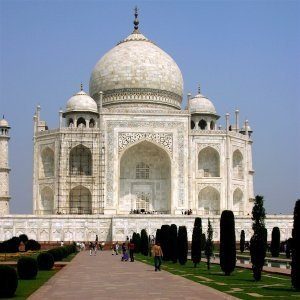
\includegraphics{figs/blur_gaussian_original.jpg}}
    	\subfigure[处理后]{
    		\label{filters:render:pattern:jigsaw:figure:dealt}
    		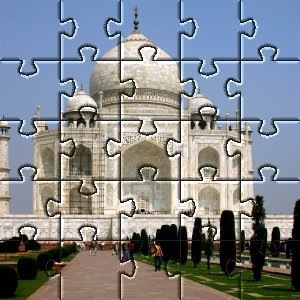
\includegraphics{figs/render_pattern_jigsaw_dealt.jpg}}
    	\label{filters:render:pattern:jigsaw:figure}
\end{figure}
\clearpage


\subsubsection{Gfig滤镜}\label{filters:render:gfig}
Gfig滤镜是一个工具:你可以用它创建几何图形并加入到图片中。当使用这个滤镜的时候,将要被插入到图像中的元素将被放置到一个新的图层。所以原先的图像不会被修改,所有的修改只会作用在新图层。\\
对话框参数设置:
\begin{description}
\item[笔画]	选中该选项时,可以选择颜色以及笔刷。
\item[填充]	选择给对象填充颜色,图案还是渐变。
\end{description}
Gfig滤镜效果如下图\ref{filters:render:gfig:figure}
\begin{figure}[!htbp]
	\centering
	\caption{Gfig滤镜}
	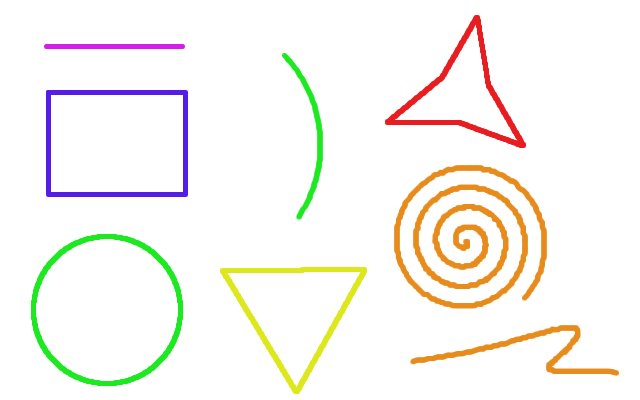
\includegraphics[scale=0.5]{figs/rendering_gfig.jpg} 
    	\label{filters:render:gfig:figure}
\end{figure}






\clearpage